\documentclass[12pt,titlepage]{article}
\usepackage[margin=1.25in]{geometry}
\usepackage{graphicx,amsmath,blindtext,minted}

%% Variables definition
\newcommand{\vSubject}{Data Structure and Algorithm Practicum}
\newcommand{\vSubtitle}{Brute Force and Divide Conquer}
\newcommand{\vName}{Muhammad Baihaqi Aulia Asy'ari}
\newcommand{\vNIM}{2241720145}
\newcommand{\vClass}{1I}
\newcommand{\vDepartment}{Information Technology}
\newcommand{\vStudyProgram}{D4 Informatics Engineering}

%% [START] Tikz related stuff
\usepackage{tikz}
\usetikzlibrary{svg.path,calc,shapes.geometric,shapes.misc}
\tikzstyle{terminator} = [rectangle, draw, text centered, rounded corners = 1em, minimum height=2em]
\tikzstyle{preparation} = [chamfered rectangle, chamfered rectangle sep=0.75em, draw, text centered, minimum height = 2em]
\tikzstyle{process} = [rectangle, draw, text centered, minimum height=2em]
\tikzstyle{decision} = [diamond, aspect=2, draw, text centered, minimum height=2em]
\tikzstyle{data}=[trapezium, draw, text centered, trapezium left angle=60, trapezium right angle=120, minimum height=2em]
\tikzstyle{connector} = [line width=0.25mm,->]
%% [END] Tikz related stuff

%% [START] Fancy header related stuff
\usepackage{fancyhdr}
\pagestyle{fancy}
\setlength{\headheight}{15pt} % compensate fancyhdr style
\fancyhead{}
\fancyfoot{}
\fancyfoot[L]{\thepage}
\fancyfoot[R]{\textit{\vSubject - \vSubtitle}}
\renewcommand{\footrulewidth}{0.4pt}% default is 0pt, overline for footer
%% [END] Fancy header related stuff

%% [START] Custom tabular command related stuff
\usepackage{tabularx}
\newcommand{\details}[2]{
    #1 & #2  \\
}
%% [END] Custom tabular command related stuff

%% [START] Figure related stuff
\newcommand{\image}[3][1]{
    \begin{figure}[h]
        \centering
        \includegraphics[#1]{#2}
        \caption{#3}
        \label{#3}
    \end{figure}
}
%% [END] Figure related stuff

%%
\usepackage{pgf-umlcd}

\renewcommand{\umldrawcolor}{black}
\renewcommand{\umlfillcolor}{white}
%%

%% [BEGIN] Custom enumerator
\usepackage{enumitem}
%% [END] Custom enumerator

\begin{document}
\begin{titlepage}
    \centering
    \vfill
    {\bfseries\LARGE
        \vSubject\\
        \vskip0.25cm
        \vSubtitle
    }
    \vfill
    
\includegraphics[width=6cm]{images/polinema-logo.png}
    \vfill
    {
        \textbf{Name}\\
        \vName\\
        \vskip0.5cm
        \textbf{NIM}\\
        \vNIM\\
        \vskip0.5cm
        \textbf{Class}\\
        \vClass\\
        \vskip0.5cm
        \textbf{Department}\\
        \vDepartment\\
        \vskip0.5cm
        \textbf{Study Program}\\
        \vStudyProgram
    }
\end{titlepage}

\newpage

\setcounter{section}{2}

\subsection{Purpose}

\begin{enumerate}
    \item Students know about the use of the brute force algorithm and the devide-conquer algorithm
    \item Students are able to apply the use of the brute force and devide-conquer algorithms
\end{enumerate}

\subsection{Theory}
Computational problem solving can be solved in various ways. Brute force and divide conquer algorithms are two different types of approaches that are usually used in problem solving.

\subsubsection{Brute Force}
Brute force is a straightforward approach to solving a problem. The basis for solving the brute force algorithm is obtained from the statement of the problem (problem statement) and the definition of the concepts involved. The brute force algorithm solves problems very simply, directly, clearly.
Brute force algorithms are generally not "smart" and not efficient, because they require a large amount of computation and a long time to complete. Sometimes the brute force algorithm is also called a naive algorithm. Brute force algorithm is more suitable for small problems because it is easy to implement and simple procedures. Brute force algorithms are often used as a basis for comparison with more sophisticated algorithms. Although it is not a good method, almost all problems can be solved using the brute force algorithm. There are several weaknesses and strengths of the brute force algorithm:
    Advatages:
    \begin{enumerate}
        \item The brute force method can be used to solve most problems (wide applicability).
        \item The brute force method is simple and easy to understand.
        \item The brute force method produces a decent algorithm for several important problems such as searching, sorting, string matching, matrix multiplication.
        \item The brute force method produces a standardized algorithm for computational tasks such as the addition / multiplication of n numbers, determining the minimum or maximum elements in a table (list).
    \end{enumerate}
    Weakness:
    \begin{enumerate}
        \item The brute force method rarely produces efficient algorithms.
        \item Some brute force algorithms are slow so that they cannot be accepted.
        \item Not as constructive / creative as other problem solving techniques.
    \end{enumerate}
Bruteforce can also be implemented in searching and sorting methods which will be explained in more detail in the following weeks. In the searching process, the principle of completion with the bruteforce method can be seen in the sequential search method. Sequential Search is also called Linear Search. The search process compares key values with all value elements. Compare key values with the first element to the last element, or, The process stops if the key value matches the element value without having to compare all elements.
As for sorting, bruteforce is used as the basic principle of the stages of the bubble sort and selection sort methods. The Bubble Sort algorithm is a sorting process that gradually moves to the right position (Bubble). This algorithm will sort the data from the largest to the smallest (ascending) or vice versa (descending). Simply stated, the Bubble Sort algorithm can be defined as sorting by exchanging data with the data next to it continuously until there is no change in one iteration. The selection sort method is an improvement of the bubble sort method by reducing the number of comparisons. Selection sort is a sorting method by finding the smallest data values starting from data in position 0 to position N-1. If there are N data and data collected from sequence 0 to N-1 then the sorting algorithm with the selection sort method is as follows: 1. Find the smallest data in the interval j = 0 to j = N-1 2. If at the post position is found the smallest data, exchange the data in the pos position with the data in position i if k. 3. Repeat steps 1 and 2 with j = j + i until j = N-1, and so on until j = N - 1.

\subsubsection{Divide Conquer}
Divide and Conquer was originally a military strategy known as divide ut imperes. Now the strategy is a fundamental strategy in computer science called Divide and Conquer. Divide means dividing the problem into several problems that have similarities to the original problem but are smaller in size (ideally about the same size), Conquer is a way to solve (solve) each one recursively, and Combine whose goal is to combine the solutions of each problem thus forming the original problem solution. The object of the problem, divided into input (input) or instances of size n such as:
\begin{itemize}
    \item table (array),
    \item matrix,
    \item exponent,
    \item etc., depending on the problem.
\end{itemize}
The stages of divide, conquer and combine can be seen in the image below.
\mbox{}\\
\begin{center}
    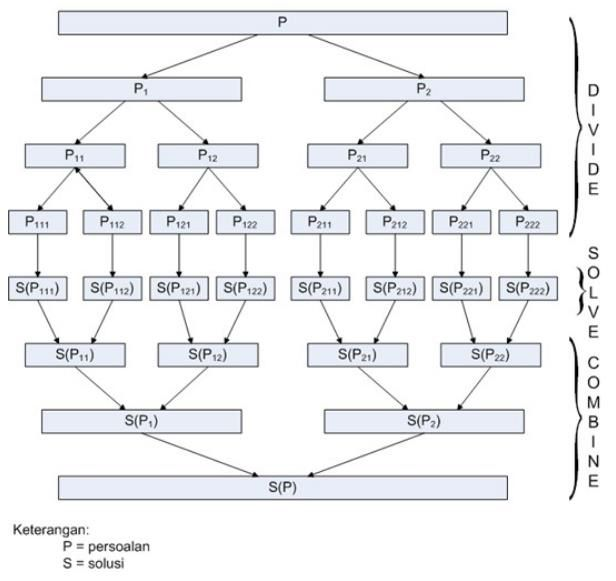
\includegraphics[width=13cm]{./images/figures/fig1.jpg}
\end{center}
\mbox{}\\
Each problem has the same characteristics as the original problem, so the Divide and Conquer method is more naturally expressed in a recursive scheme. The general pseudocode for solving problems with the divide conquer algorithm is:
\begin{minted}[autogobble]{text}
        procedure DIVIDE_and_CONQUER(input n : integer)
        { Resolve problems with the D-and-C algorithm.
            Input: input size n
            Output: the solution of the original problem }
        Declaration
                r, k : integer
        Algorithm
            if n <= n0 then { the size of the problem is small enough }
                SOLVE this n-sized sub-problem
            else
                Divide r into sub-problems, each of which is sized n / k
                for each of the likeness-problems do
                    DIVIDE_and_CONQUER(n/k)
                endfor
                COMBINE the solution of the problem solution becomes the original
    problem solution
            endif

\end{minted}
Weakness Divide and Conquer

\begin{itemize}
    \item Slow iteration process
    \begin{itemize}
        \item Slow looping The process of calling sub-routine (can slow down the looping process) will cause excessive call stack full. This can be a significant burden on the processor. More complicated for simple problems
    \end{itemize}
    \item More complicated for simple problems
    \begin{itemize}
        \item For simple problem solving, a sequential algorithm is proven to be easier to create than the divide and conquer algorithm.
    \end{itemize}
\end{itemize}

Advantages of Divide and Conquer

\begin{itemize}
    \item Can solve difficult problems. Solving Divide and Conquer problems is a very effective way if the problem to be solved is complicated enough.
    \item Has high algorithmic efficiency. This divide and conquer approach is more efficient in completing the sorting algorithm.
    \item Can work in parallel. Divide and Conquer has been designed to work on machines that have multiple processors. Especially machines that have a memory sharing system, where data communication between processors does not need to be planned in advance, this is because solving sub-routines can be done on other processors.
    \item Memory access is quite small. For memory access, Divide and Conquer can improve the efficiency of existing memory quite well. This is because, sub-routine requires less memory than the main problem.
\end{itemize}

Divide conquer is also the basis for searching and sorting. The sorting method that uses basic divide conquer is merge sort. The sorting method for merge sort is the advanced sorting method, the same as the Quick Sort method. This method also uses the concept of devide and conquer which divides S data into two groups, namely S1 and S2 which are not intersected (disjoint). The process of data sharing is done recursively until the data cannot be divided again or in ot the data in sub sections becomes single. After the data cannot be divided again, the me process is carried out between sub-sections by paying attention to the desired data sequence (ascending / small to large or descending / large to small). This merging process is carried out until all data is combined and ordered in the desired order. While searching methods that use a way of sharing solutions such as divide conquere is binary search. Binary search is an algorithm for passing searches in an ordered array. If we do not know how integer information is in an array, then the use of binary search will be inefficient, we must sort first or use another method, namely linear search. But if we already know that integers in organized arrays are either ascending or descending, then we can quickly use the binary search algorithm.

\subsection{Calculating Factorial Values with Brute Force and Divide and Conquer Algorithms}
Consider the following Class Diagram:
\mbox{}\\
    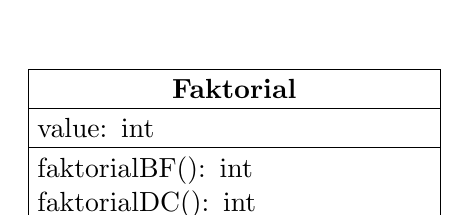
\begin{tikzpicture}
        \begin{class}[text width=5cm]{Faktorial}{0,0}
            \attribute{value: int}
            \operation{faktorialBF(): int}
            \operation{faktorialDC(): int}
        \end{class}
    \end{tikzpicture}
\mbox{}\\
Based on the class diagram above, a class program will be created in Java. To calculate the factorial value of a number using 2 types of algorithms, Brute Force and Divide and Conquer. If described there are differences in the calculation process of the 2 types of algorithm as follows:
\mbox{}\\
The stages of factorial value searching with Brute Force algorithm:
\mbox{}\\
\includegraphics[]{./images/figures/fig2.jpg}
\mbox{}\\
The stages of factorial value searching with the Divide and Conquer algorithm:
\mbox{}\\
\includegraphics[]{./images/figures/fig3.jpg}

\subsubsection{Practicum}

\begin{enumerate}
    \item Create a new Project, with the name AlgoStruDat / Project Name Equated to last week. Make a package with the name \textbf{Week3}, make a new class with the name \textbf{Faktorial}.
    \item Complete the Faktorial class with the attributes and methods described in the class diagram above:
    \begin{enumerate}
        \item Add value attributes
        \begin{minted}[autogobble,breaklines]{java}
            public int num;
        \end{minted}
        \item Add method \texttt{faktorialBF()}
        \begin{minted}[autogobble,breaklines]{java}
            public int faktorialBF(int n) {
                int fakto = 1;
                for (int i = 1; i <= n; i++) {
                    fakto = fakto * i;
                }
                return fakto;
            }
        \end{minted}
        \item Add method \texttt{faktorialDC()}
        \begin{minted}[autogobble,breaklines]{java}
            public int faktorialDC(int n) {
                if (n==1) {
                    return 1;
                }
                else
                {
                    int fakto = n * faktorialDC(n-1);
                    return fakto;
                }
            }
        \end{minted}
    \end{enumerate}
    \item Run the \texttt{Faktorial class} y creating a new \texttt{MainFaktorial} class.
    \begin{enumerate}
        \item In the main function, provide input to input the number of numbers to find the factorial value
        \begin{minted}[autogobble,breaklines]{java}
            Scanner sc = new Scanner(System.in);
            System.out.println("================================ ================================");
            System.out.print("Input the number of elements you want to count : ");
            int elemen = sc.nextInt();
        \end{minted}
        \item Create an Array of Objects on the main function, then input some values that will be factorially calculated
        \begin{minted}[autogobble,breaklines]{java}
            Faktorial [] fk = new Faktorial[elemen];
            for (int i = 0; i < elemen; i++) {
                fk[i] = new Factorial();
                System.out.print("Input the data value to-"+(i+1)+" : ");
                fk[i].num = sc.nextInt();
            }
        \end{minted}
        \item Display the results of calling method \texttt{faktorialDC()} dan \texttt{faktorialBF()}
        \begin{minted}[autogobble,breaklines]{java}
            System.out.println("================================ ================================");
            System.out.println("Factorial Result with Brute Force");
            for (int i = 0; i < elemen; i++) {
                System.out.println("Factorial of value"+fk[i].num+" is : "+fk[i].faktorialBF(fk[i].num));
            }
            
            System.out.println("================================ ================================");
            for (int i = 0; i < elemen; i++) {
                System.out.println("Factorial of value"+fk[i].num+" is : "+fk[i].faktorialDC(fk[i].num));
            }
            System.out.println("================================ ================================");
        \end{minted}
        \item Make sure the program is running well!
    \end{enumerate}
\end{enumerate}

\begin{enumerate}
    \item \texttt{Faktorial.java}
    \begin{minted}[autogobble,breaklines]{java}
        package Faktorial;

        public class Faktorial {
            public int num;
            public int faktorialBF(int n) {
                int fakto = 1;
                for (int i = 1; i <= n; i++) {
                    fakto = fakto * i;
                }
                return fakto;
            }
            public int faktorialDC(int n) {
                if (n==1) {
                    return 1;
                }
                else
                {
                    int fakto = n * faktorialDC(n-1);
                    return fakto;
                }
            }
        }
    \end{minted}
    \item \texttt{MainFaktorial.java}
    \begin{minted}[autogobble,breaklines]{java}
        package Faktorial;

        public class MainFaktorial {
            public static void main(String[] args) {
                Scanner sc = new Scanner(System.in);
                    System.out.println("================================ ================================");
                    System.out.print("Input the number of elements you want to count : ");
                    int elemen = sc.nextInt();
                    Faktorial [] fk = new Faktorial[elemen];
                    for (int i = 0; i < elemen; i++) {
                        fk[i] = new Factorial();
                        System.out.print("Input the data value to-"+(i+1)+" : ");
                        fk[i].num = sc.nextInt();
                    }
                    System.out.println("================================ ================================");
                    System.out.println("Factorial Result with Brute Force");
                    for (int i = 0; i < elemen; i++) {
                        System.out.println("Factorial of value "+fk[i].num+" is : "+fk[i].faktorialBF(fk[i].num));
                    }
                    
                    System.out.println("================================ ================================");
                    for (int i = 0; i < elemen; i++) {
                        System.out.println("Factorial of value "+fk[i].num+" is : "+fk[i].faktorialDC(fk[i].num));
                    }
                    System.out.println("================================ ================================");
            }
        }
    \end{minted}
\end{enumerate}

\subsubsection{Verification of Practicum Results}

\begin{minted}[autogobble,breaklines]{text}
    ================================================================
    Input the number of elements you want to count : 3
    Input the data value to-1 : 5
    Input the data value to-2 : 8
    Input the data value to-3 : 3
    ================================================================
    Factorial Results with Brute Force
    Factorial of value 5 : 120
    Factorial of value 8 : 40320
    Factorial of value 3 : 6
    ================================================================
    Factorial Results with Divide and Conquer
    Factorial of value 5 : 120
    Factorial of value 8 : 40320
    Factorial of value 3 : 6
    ================================================================
\end{minted}

\texttt{Result: }

\begin{minted}[autogobble,breaklines,linenos]{text}
    PS D:\Kuliah>  d:; cd 'd:\Kuliah'; & 'C:\Program Files\Java\jdk-18.0.2.1\bin\java.exe' '-XX:+ShowCodeDetailsInExceptionMessages' '-cp' 'C:\Users\ASUS\AppData\Roaming\Code\User\workspaceStorage\ ce3fcb236261368a6cbd019dc8ddda8b\redhat.java\jdt_ws\ Kuliah_28156aa7\bin' 'Faktorial.MainFaktorial' 
    ================================================================
    Input the number of elements you want to count : 3
    Input the data value to-1 : 5
    Input the data value to-2 : 8
    Input the data value to-3 : 3
    ================================================================
    Factorial Result with Brute Force
    Factorial of value 5 is : 120
    Factorial of value 8 is : 40320
    Factorial of value 3 is : 6
    ================================================================
    Factorial of value 5 is : 120
    Factorial of value 8 is : 40320
    Factorial of value 3 is : 6
    ================================================================
\end{minted}

\subsubsection{Questions}

\begin{enumerate}
    \item Explain the Divide Conquer Algorithm for calculating factorial values!
    \mbox{}\\
    \texttt{Answer: }
    \mbox{}\\
    The algorithm check if the parameter is 1. If it is, it will return 1. When the parameter anything else but 1, then it will calculate the parameter multiplied by the return of factorial divide and conquer function with the parameter of the original parameter minus one and then return the result of that calculation. Because of this any number else then one will recursively call it self with the parameter number minus one than before until the parameter becomes one.
    \item In the implementation of Factorial Divide and Conquer Algorithm is it complete that consists of 3 stages of divide, conquer, combine? Explain each part of the program code!
    \mbox{}\\
    \texttt{Answer: }
    \mbox{}\\ .
    \mbox{}
    The divide stage is implemented when the factorialDC function call it self. When a recursion happend the process of the previous function call is halted until the current function calculate has return a value. These function call happend until the function met its halting condition. 
    \mbox{}\\ .
    \mbox{}
    The conquer stage is process when the function calls has collaps on itself after meeting its halting condition. The function collaps by returning value from the function with halting condition as its parameter. 
    \mbox{}\\ .
    \mbox{}
    The combine stage happend when the function is processing its return value. The return value of the function is calculated before the value is sent to the previous function call. The previous function call will aslo do the same thing until there is no more function waiting for a value or to put it in another term the function will stop collaps on itself when it has reach the first call function on the stack.
    \item Is it possible to repeat the factorial BF() method instead of using for? Prove it!
    \mbox{}\\
    \texttt{Answer: }
    \mbox{}\\
    Yes.
    \begin{minted}[autogobble,breaklines]{java}
        public int faktorialBF(int n) {
            int fakto = 1;
            int i = 0;
            While(i <= n) {
                fakto = fakto * i;
                i++
            }
            return fakto;
        }
    \end{minted}
    \item Add a check to the execution time of the two types of methods!
    \begin{minted}[autogobble,breaklines]{java}
        package Faktorial;

        import java.util.Scanner;

        public class MainFaktorial {
            public static void main(String[] args) {
                Scanner sc = new Scanner(System.in);
                    System.out.println("================================ ================================");
                    System.out.print("Input the number of elements you want to count : ");
                    int elemen = sc.nextInt();
                    Faktorial [] fk = new Faktorial[elemen];
                    for (int i = 0; i < elemen; i++) {
                        fk[i] = new Faktorial();
                        System.out.print("Input the data value to-"+(i+1)+" : ");
                        fk[i].num = sc.nextLong(10);
                    }
                    System.out.println("================================ ================================");
                    System.out.println("Factorial Result with Brute Force");
                    for (int i = 0; i < elemen; i++) {
                        long faktorialBFStart = System.nanoTime();
                        System.out.println("Factorial of value "+fk[i].num+" is : "+fk[i].faktorialBF(fk[i].num));
                        long faktorialBFEnd = System.nanoTime();
                        System.out.printf("Time in nanoseconds: %,d\n",faktorialBFEnd - faktorialBFStart);
                    }
                    
                    System.out.println("================================ ================================");
                    System.out.println("Factorial Result with Divide and Conquer");
                    for (int i = 0; i < elemen; i++) {
                        long faktorialDCStart = System.nanoTime();
                        System.out.println("Factorial of value "+fk[i].num+" is : "+fk[i].faktorialDC(fk[i].num));
                        long faktorialDCEnd = System.nanoTime();
                        System.out.printf("Time in nanoseconds: %,d\n",faktorialDCEnd-faktorialDCStart);
                    }
                    System.out.println("================================ ================================");

                    sc.close();
            }
        }
    \end{minted}
    \item Prove by inputting elements that are above 20 digits, is there a difference in execution time?
    \begin{minted}[autogobble,breaklines,linenos]{text}
        PS D:\Kuliah>  d:; cd 'd:\Kuliah'; & 'C:\Program Files\Java\jdk-18.0.2.1\bin\java.exe' '-XX:+ShowCodeDetailsInExceptionMessages' '-cp' 'C:\Users\G4CE-PC\AppData\Roaming\Code\User\workspaceStorage\ 80d97a47d24665dc0bce7ab1e048ecbd\redhat.java\jdt_ws\ Kuliah_28156aa7\bin' 'Faktorial.MainFaktorial' 
        ================================================================
        Input the number of elements you want to count : 1
        Input the data value to-1 : 50
        ================================================================
        Factorial Result with Brute Force
        Factorial of value 50 is : -3258495067890909184
        Time in nanoseconds: 335,000
        ================================================================
        Factorial Result with Divide and Conquer
        Factorial of value 50 is : -3258495067890909184
        Time in nanoseconds: 172,100
        ================================================================ 
    \end{minted}
    Yes, there is. With bigger base number, the difference in time rise.
\end{enumerate}

\subsection{Calculating Squared Results with Brute Force and Divide and Conquer Algorithms}

\subsubsection{Practicum}

\begin{enumerate}
    \item In the week 3 package, create a new class named Squared, then create the num attribute that will be raised with the squared number
    \begin{minted}[autogobble,breaklines]{java}
        public int num, squared;
    \end{minted}
    \item In the Squared class, add the SquaredBF() method
    \begin{minted}[autogobble,breaklines]{java}
        public int squaredBF(int a, int n) {
            int result = 1;
            for (int i = 0; i < n; i++) {
                result = result * a;
            }
            return result;
        }
    \end{minted}
    \item In the Squared class also add a method SquaredDC()
    \begin{minted}[autogobble,breaklines]{java}
        public int squaredDC(int a, int n) {
            if (n == 0) {
                return 1;
            } else {
                if (n % 2 == 1) {
                    return (squaredDC(a, n/2) * squaredDC(a, n/2) * a);
                } else {
                    return (squaredDC(a, n/2) * squaredDC(a, n/2));
                }
            }
        }
    \end{minted}
    \item Observe whether there are no errors that appear in the making of the Squared class
    \item Next create a new class in which there is a main method. This class can be called MainSquared. Add code to the main class to input the number of values to be counted.
    \begin{minted}[autogobble,breaklines]{java}
        Scanner sc = new Scanner(System.in);
        System.out.println("================================================");
        System.out.print("Input the number of elements you want to count : ");
        int elemen = sc.nextInt();
    \end{minted}
    \item The values in step 5 are then used for the instantiation of arrays of objects. The following code is added to the process of filling in some values which will be raised to the squared.
    \begin{minted}[autogobble,breaklines]{java}
        Squared[] png = new Squared[elemen];
        
        for (int i = 0; i < elemen; i++) {
            png[i] = new Squared();
            System.out.print("Input the value to be squared to-"+(i+1)+" : ");
            png[i].num = sc.nextInt();
            System.out.print("Input the squared value to-"+(i+1)+" : ");
            png[i].squared = sc.nextInt();
        }
    \end{minted}
    \item Call the results by returning the return value of the method SquaredBF() dan SquaredDC().
    \begin{minted}[autogobble,breaklines]{java}
        System.out.println("================================================");
        System.out.println("Results with Brute Force Squared");
        for (int i = 0; i < elemen; i++) {
            System.out.println("Value "+png[i].num+" squared "+png[i].squared+" is : "+png[i].squaredBF(png[i].num, png[i].squared));
        }
        System.out.println("================================================");
        System.out.println("Results with Divide and Conquer Squared");
        for (int i = 0; i < elemen; i++) {
            System.out.println("Value "+png[i].num+" squared "+png[i].squared+" is : "+png[i].squaredDC(png[i].num, png[i].squared));
        }
        System.out.println("================================================");
    \end{minted}
\end{enumerate}

\subsubsection{Verification of Practicum Results}

\begin{minted}[autogobble,breaklines,linenos]{text}
    PS D:\Kuliah>  & 'C:\Program Files\Java\jdk-18.0.2.1\bin\java.exe' '-XX:+ShowCodeDetailsInExceptionMessages' '-cp' 'C:\Users\G4CE-PC\AppData\Roaming\Code\User\workspaceStorage\ 80d97a47d24665dc0bce7ab1e048ecbd\redhat.java\jdt_ws\ Kuliah_28156aa7\bin' 'Faktorial.MainSquared'
    ================================================
    Input the number of elements you want to count : 2
    Input the value to be squared to-1 : 6
    Input the squared value to-1 : 2
    Input the value to be squared to-2 : 4
    Input the squared value to-2 : 3
    ================================================
    Results with Brute Force Squared
    Value 6 squared 2 is : 36
    Value 4 squared 3 is : 64
    ================================================
    Results with Divide and Conquer Squared
    Value 6 squared 2 is : 36
    Value 4 squared 3 is : 64
    ================================================
\end{minted}

\subsubsection{Questions}

\begin{enumerate}
    \item Explain the differences between the 2 methods made are SquaredBF() and SquaredDC()!
    \mbox{}\\
    \texttt{Answer: }
    \mbox{}\\
    BF loops the base number trough the exponent. Meanwhile the DC divide the problem into smaller problem before combining the result.
    \item In the SuaredDC() method there is a program as follows:
    \begin{minted}[autogobble,breaklines]{java}
        if (n % 2 == 1) {
            return (squaredDC(a, n/2) * squaredDC(a, n/2) * a);
        } else {
            return (squaredDC(a, n/2) * squaredDC(a, n/2));
        }
    \end{minted}
    Explain the meaning of the code!
    \texttt{Answer: }
    \mbox{}\\
    If the exponent of the problem is odd, it will process the problem by dividing it into 2 function and a multiplication with the base number. If the exponent number is even, it will just divide the problem into 2 function.
    \item Explain whether the combine stage is included in the code!
    \mbox{}\\
    \texttt{Answer: }
    \mbox{}\\
    It is included, as the division of the problem contain a process of combining the solution from the sub-problems.
    \item Modification of the program code, assuming the attribute filling process is done by a constructor.
    \begin{minted}[autogobble,breaklines]{java}
        package Faktorial;

        import java.util.Scanner;

        public class MainSquared {
            public static void main(String[] args) {
                Scanner sc = new Scanner(System.in);
                System.out.println("================================================");
                System.out.print("Input the number of elements you want to count : ");
                int elemen = sc.nextInt();
                
                Squared[] png = new Squared[elemen];
                
                for (int i = 0; i < elemen; i++) {
                    System.out.print("Input the value to be squared to-"+(i+1)+" : ");
                    int num = sc.nextInt();
                    System.out.print("Input the squared value to-"+(i+1)+" : ");
                    int squared = sc.nextInt();
                    png[i] = new Squared(num, squared);
                }

                System.out.println("================================================");
                System.out.println("Results with Brute Force Squared");
                for (int i = 0; i < elemen; i++) {
                    System.out.println("Value "+png[i].num+" squared "+png[i].squared+" is : "+png[i].squaredBF(png[i].num, png[i].squared));
                }
                System.out.println("================================================");
                System.out.println("Results with Divide and Conquer Squared");
                for (int i = 0; i < elemen; i++) {
                    System.out.println("Value "+png[i].num+" squared "+png[i].squared+" is : "+png[i].squaredDC(png[i].num, png[i].squared));
                }
                System.out.println("================================================");

                sc.close();
            }
        }
    \end{minted}
    \item Add a menu so that only one of the selected methods will be run!
    \begin{minted}[autogobble,breaklines]{java}
        package Faktorial;

        import java.util.Scanner;

        public class MainSquared {
            static Scanner sc = new Scanner(System.in);
            static int globalElemen;
            static Squared[] globalPng;

            static void callBF() {
                System.out.println("================================================");
                System.out.println("Results with Brute Force Squared");
                for (int i = 0; i < globalElemen; i++) {
                    System.out.println("Value "+globalPng[i].num+" squared "+globalPng[i].squared+" is : "+globalPng[i].squaredBF(globalPng[i].num, globalPng[i].squared));
                }
                System.out.println("================================================");
            }

            static void callDC() {
                System.out.println("================================================");
                System.out.println("Results with Divide and Conquer Squared");
                for (int i = 0; i < globalElemen; i++) {
                    System.out.println("Value "+globalPng[i].num+" squared "+globalPng[i].squared+" is : "+globalPng[i].squaredDC(globalPng[i].num, globalPng[i].squared));
                }
                System.out.println("================================================");
            }
            public static void main(String[] args) {
                System.out.println("================================================");
                System.out.print("Input the number of elements you want to count : ");
                int elemen = sc.nextInt();
                Squared[] png = new Squared[elemen];

                globalElemen = elemen;
                globalPng = png;
                
                
                for (int i = 0; i < elemen; i++) {
                    System.out.print("Input the value to be squared to-"+(i+1)+" : ");
                    int num = sc.nextInt();
                    System.out.print("Input the squared value to-"+(i+1)+" : ");
                    int squared = sc.nextInt();
                    png[i] = new Squared(num, squared);
                }

                boolean choosen = false;
                System.out.println("Choose the algorithm");
                System.out.println("1. Brute Force");
                System.out.println("2. Divide and Conquer");
                while (!choosen) {
                    System.out.print("Menu: ");
                    sc.nextLine();
                    char menu = sc.nextLine().charAt(0);

                    switch (menu) {
                        case '1':
                            choosen = true;
                            callBF();
                            break;

                        case '2':
                            choosen = true;
                            callDC();
                            break;

                        default:
                            System.out.println("Please enter the number available in the option");
                            break;
                    }
                }


                sc.close();
            }
        }
    \end{minted}
\end{enumerate}

\subsection{Calculating Sum Array with Brute Force and Divide and Conquer Algorithms}
In this practicum, we will practice how the divide, conquer, and combine process is applied to a case study of the sum of profits of a company in a few months.

\subsubsection{Practicum}

\begin{enumerate}
    \item On week package3. Create a new class, the Sum class. IN the class Sum there are several attributes of the number of array elements, arrays, and total.
    \begin{minted}[autogobble,breaklines]{java}
        public int elemen;
        public double profit[];
        public double total;
    \end{minted}
    \item Add the constructor Sum() with the parameter int elemen
    \begin{minted}[autogobble,breaklines]{java}
        public Sum(int element) {
            elemen = element;
            profit = new double[elemen];
            total = 0;
        }
    \end{minted}
    \item Add the TotalBF() method which will calculate the total value of the array with iterative.
    \begin{minted}[autogobble,breaklines]{java}
        double totalBF(double arr[]) {
            for (int i = 0; i < elemen; i++) {
                total = total + arr[i];
            }
            return total;
        }
    \end{minted}
    \item Add the TotalDC() method to implement the calculation of the total array value using the Divide and Conquer algorithm
    \begin{minted}[autogobble,breaklines]{java}
        double totalDC(double arr[], int l, int r) {
            if (l==r) {
                return arr[l];
            } else if (l < r) {
                int mid = (l+r)/2;
                double lsum = totalDC(arr, l, mid-1);
                double rsum =  totalDC(arr, mid + 1, r);
                return lsum+rsum+arr[mid];
            }
            return 0;
        }
    \end{minted}
    \item In this class there is a main method. In this method the user can write how many months the profit will be calculated. In this class an object instance is also created to call the attributes or functions of the Sum class
    \begin{minted}[autogobble,breaklines]{java}
        Scanner sc = new Scanner(System.in);
        System.out.println("================================ ================================");
        System.out.println("Program for Calculating Total Profits");
        System.out.println("Input the Number of Months : ");
        int totElemen = sc.nextInt();
        Sum sm = new Sum(totElemen);
        sm.elemen = totElemen;
    \end{minted}
    \item Make a loop to fill the profit amount according to the number of months entered (fill in the profit value to each array index)
    \begin{minted}[autogobble,breaklines]{java}
        System.out.println("================================ ================================");
        for (int i = 0; i < sm.elemen; i++) {
            System.out.print("Input the profit of the month to - "+(i+1)+" = ");
            sm.profit[i] = sc.nextDouble();
        }
    \end{minted}
    \item Show the results of calculations through objects that have been made for both algorithm (Brute Force and Divide Conquer) by calling the totalBF() and totalDF() methods of the Sum class.
    \begin{minted}[autogobble,breaklines]{java}
        System.out.println("================================ ================================");
        System.out.println("Algoritma Brute Force");
        System.out.println("Total profits of the company for " + sm.elemen + " month is = " + sm.totalBF(sm.profit));
        System.out.println("================================ ================================");
        System.out.println("Algoritma Divide Conquer");
        System.out.println("Total profits of the company for " + sm.elemen + " month is = " + sm.totalDC(sm.profit, 0, sm.elemen-1));
    \end{minted}
    \texttt{Result: }
    \begin{minted}[autogobble,breaklines]{java}
        package Bfndc;

        public class Sum {
            public int elemen;
            public double profit[];
            public double total;

            public Sum(int element) {
                elemen = element;
                profit = new double[elemen];
                total = 0;
            }

            double totalBF(double arr[]) {
                for (int i = 0; i < elemen; i++) {
                    total = total + arr[i];
                }
                return total;
            }

            double totalDC(double arr[], int l, int r) {
                if (l==r) {
                    return arr[l];
                } else if (l < r) {
                    int mid = (l+r)/2;
                    double lsum = totalDC(arr, l, mid-1);
                    double rsum =  totalDC(arr, mid + 1, r);
                    return lsum+rsum+arr[mid];
                }
                return 0;
            }
        }
    \end{minted}
    \begin{minted}[autogobble,breaklines]{java}
        package Bfndc;

        import java.util.Scanner;

        public class MainSum {
            public static void main(String[] args) {
                Scanner sc = new Scanner(System.in);
                System.out.println("================================ ================================");
                System.out.println("Program for Calculating Total Profits");
                System.out.println("Input the Number of Months : ");
                int totElemen = sc.nextInt();
                Sum sm = new Sum(totElemen);
                sm.elemen = totElemen;
                
                System.out.println("================================ ================================");
                for (int i = 0; i < sm.elemen; i++) {
                    System.out.print("Input the profit of the month to - "+(i+1)+" = ");
                    sm.profit[i] = sc.nextDouble();
                }

                System.out.println("================================ ================================");
                System.out.println("Algoritma Brute Force");
                System.out.println("Total profits of the company for " + sm.elemen + " month is = " + sm.totalBF(sm.profit));
                System.out.println("================================ ================================");
                System.out.println("Algoritma Divide Conquer");
                System.out.println("Total profits of the company for " + sm.elemen + " month is = " + sm.totalDC(sm.profit, 0, sm.elemen-1));
                
                sc.close();
            }
        }

    \end{minted}
\end{enumerate}

\subsubsection{}

\begin{minted}[autogobble,breaklines,linenos]{text}
    PS D:\Kuliah>  d:; cd 'd:\Kuliah'; & 'C:\Program Files\Java\jdk-18.0.2.1\bin\java.exe' '-XX:+ShowCodeDetailsInExceptionMessages' '-cp' 'C:\Users\G4CE-PC\AppData\Roaming\Code\User\workspaceStorage\80d97a47d24665dc0bce7ab1e048ecbd\redhat.java\jdt_ws\Kuliah_28156aa7\bin' 'Bfndc.MainSum' 
    ================================================================
    Program for Calculating Total Profits
    Input the Number of Months :
    4
    ================================================================
    Input the profit of the month to - 1 = 1000
    Input the profit of the month to - 2 = 2000
    Input the profit of the month to - 3 = 3000
    Input the profit of the month to - 4 = 1000
    ================================================================
    Algoritma Brute Force
    Total profits of the company for 4 month is = 7000.0
    ================================================================
    Algoritma Divide Conquer
    Total profits of the company for 4 month is = 7000.0
\end{minted}

\subsubsection{Questions}

\begin{enumerate}
    \item Give an illustration of the difference in profit calculation with the TotalBF() or TotalDC() method.
    \mbox{}\\
    \texttt{Answer:}
    \mbox{}\\
    The TotalBF iterate and add. Meanwhile TotalDC divide the the array by cutting the array in the middle until there is only one element in the array. After which they combine to their counter part of the split.
    \item Why is there the following return value? Explain!
    \begin{minted}[autogobble,breaklines]{java}
        return lsum+rsum+arr[mid];
    \end{minted}
    \mbox{}\\
    \texttt{Answer:}
    \mbox{}\\
    The return value is used to combine the value and return it to the function after the sub-problem function has been conquered.
    \item Why is the mid variable required for the TotalDC() method?
    \mbox{}\\
    \texttt{Answer:}
    \mbox{}\\
    Because the mid variable are going to be the last element of the array after the problem has finish dividing.
    \item The profit calculation program for a company is only for one company. How do you calculate several months of profit for several companies at once (each company can have a different number of months)? Prove it with the program!
    \mbox{}\\
    \texttt{Answer:}
    \mbox{}\\
\end{enumerate}

\subsection{Assignments}

\begin{enumerate}
    \item Create a program based on the following class diagram!
    \mbox{}\\
    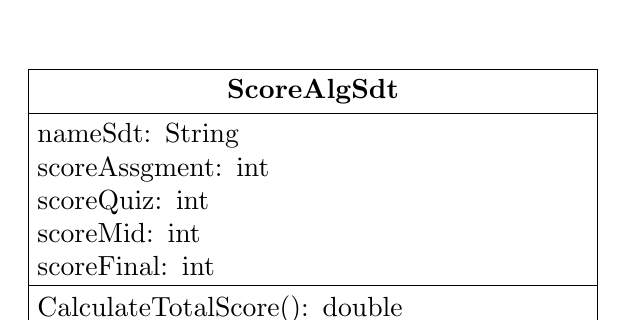
\begin{tikzpicture}
        \begin{class}[text width=7cm]{ScoreAlgSdt}{0,0}
            \attribute{nameSdt: String}
            \attribute{scoreAssgment: int}
            \attribute{scoreQuiz: int}
            \attribute{scoreMid: int}
            \attribute{scoreFinal: int}
            \operation{CalculateTotalScore(): double}
        \end{class}
    \end{tikzpicture}
    \mbox{}\\
    Score are calculated based on total Assignment of 30\%, Quiz 20\%, Mid 20\%, Final 30\%. Adjust the method if it must have parameters.
    \begin{minted}[autogobble,breaklines]{java}
        package Assignment;

        public class ScoreAlgSdt {
            String nameSdt;
            int scoreAssgnment;
            int scoreQuiz;
            int scoreMid;
            int scoreFinal;

            public ScoreAlgSdt(String nameSdt, int scoreAssgnment, int scoreQuiz, int scoreMid, int scoreFinal) {
                this.nameSdt = nameSdt;
                this.scoreAssgnment = scoreAssgnment;
                this.scoreQuiz = scoreQuiz;
                this.scoreMid = scoreMid;
                this.scoreFinal = scoreFinal;
            }

            public double calculateTotalScore() {
                return scoreAssgnment * 0.3 + scoreQuiz * 0.2 + scoreMid * 0.2 + scoreFinal * 0.3;
            }
        }
    \end{minted}
    \item (continued about question no. 1). Create an array of objects in the main class to find out the value of several students in one calculation at a time!
    \begin{minted}[autogobble,breaklines]{java}
        package Assignment;

        import java.util.Scanner;

        public class ScoreAlgSdtMain {
            public static void main(String[] args) {
                Scanner sc = new Scanner(System.in);

                System.out.print("Enter amount of student: ");
                int amount = sc.nextInt();
                ScoreAlgSdt[] scores = new ScoreAlgSdt[amount];

                for (int i = 0; i < scores.length; i++) {
                    System.out.print("");
                    String name = sc.nextLine();
                    System.out.print("");
                    int scoreAssgnment = sc.nextInt();
                    System.out.print("");
                    int scoreQuiz = sc.nextInt();
                    System.out.print("");
                    int scoreMid = sc.nextInt();
                    System.out.print("");
                    int scoreFinal = sc.nextInt();
                    scores[i] = new ScoreAlgSdt(name, scoreAssgnment, scoreQuiz, scoreMid, scoreFinal);
                }

                sc.close();
            }
        }
    \end{minted}
    \item (Continued question no. 2) with the modified Brute Force algorithm program in order to know the average value of all students who have been inputted to the Algorithm and data structure course. \mbox{}\\
    Example : \mbox{}\\
    There are a total of the following student grades
    \mbox{}\\
    \begin{tabular}{|l|l|}
        \hline
        Name & Total Value of Algorithm Courses \\
        \hline
        Rani & 86,5 \\
        \hline
        Dani & 72,5 \\
        \hline
        Saraswati & 89 \\
        \hline
        Average & 82,67 \\
        \hline
    \end{tabular}
    \mbox{}\\
    Then the average total value of all students who have taken the algorithm course is 82.67
    \begin{minted}[autogobble,breaklines]{java}
        package Assignment;

        import java.util.Scanner;

        public class ScoreAlgSdtMain {
            public static void main(String[] args) {
                Scanner sc = new Scanner(System.in);

                System.out.print("Enter amount of student: ");
                int amount = sc.nextInt();
                ScoreAlgSdt[] scores = new ScoreAlgSdt[amount];

                for (int i = 0; i < scores.length; i++) {
                    System.out.print("");
                    String name = sc.nextLine();
                    System.out.print("");
                    int scoreAssgnment = sc.nextInt();
                    System.out.print("");
                    int scoreQuiz = sc.nextInt();
                    System.out.print("");
                    int scoreMid = sc.nextInt();
                    System.out.print("");
                    int scoreFinal = sc.nextInt();
                    scores[i] = new ScoreAlgSdt(name, scoreAssgnment, scoreQuiz, scoreMid, scoreFinal);
                }
                
                double totalScore = 0; 
                for (int i = 0; i < scores.length; i++) {
                    totalScore += scores[i].calculateTotalScore();
                }
                double avgScore = totalScore/amount;

                int row =  amount + 2;
                String[] nameColumn = new String[row];
                String[] valueColumn = new String[row];

                nameColumn[0] = "Name";
                nameColumn[row-1] = "Average";
                valueColumn[0] = "Total Value of Algorithm Courses";
                valueColumn[row-1] = String.format("%,.2f", avgScore);

                for (int i = 1; i < row-1; i++) {
                    nameColumn[i] = scores[i-1].nameSdt;
                    valueColumn[i] = String.format("%,.2f", scores[i-1].calculateTotalScore());
                }

                System.out.println("There are a total of the following student grades");
                System.out.println("================================ ================================");
                for (int i = 0; i < row; i++) {
                    System.out.printf("|%s|", nameColumn[i]);
                    System.out.printf("|%s|", valueColumn[i]);
                }
                System.out.println("================================ ================================");
                System.out.printf("Then the average total value of all students who have taken the algorithm course is %,.2f", avgScore);

                sc.close();
            }
        }
    \end{minted}
    \item A university in Malang is holding a vote to elect the BEM chairman in 2020. If the number of votes collected is always even. Then by inputting the selected candidates, count the number of votes for each candidate. Make class diagrams and programs using the Divide and Conquer algorithm from the case study! (The number of array elements and the results of the vote are user input) \mbox{}\\
    Example: Voting results are as follows (m is majority, nm is not majority)
    \includegraphics[width=14cm]{./images/figures/fig4.png}
    \mbox{}\\
    Description: Blue is the divide process, yellow starts the conquer process, green starts the combining process
    \item What if the number of votes is odd? should there be a program improvement? if yes, improve the program for case study no 4. If the number of votes collected is not always even!
    \item Modify the program about the average value of algorithm courses using the Divide and Conquer Algorithm!
    
    \begin{minted}[autogobble,breaklines]{java}
        package Assignment;

        public class Vote {
            public String[] candidate;
            public int[][] votes;

            public Vote(String[] candidate) { 
                this.candidate = candidate;
            }

            public int[] count(int[][] votes, int left, int right) {
                if (left == right) {
                    int[] vote = votes[0];
                    int[] result = new int[1];
                    result[0] = sum(vote, left, right);
                    return result;
                } else {
                    int mid = (left + right) / 2;
                    int[] leftResult  = count(votes, left, mid);
                    int[] rightResult = count(votes, mid+1, right);

                    int leftLen = leftResult.length;
                    int rightLen = rightResult.length;

                    int[] result = new int[leftLen+rightLen];

                    for (int i = 0; i < leftLen; i++) {
                        result[i] = leftResult[i];
                    }
                    for (int i = leftLen; i < leftLen+rightLen; i++) {
                        result[i] = rightResult[i-leftLen];
                    }
                    return result;
                }
            }

            public int sum(int[] vote, int left, int right) {
                if (left == right) {
                    return vote[left];
                } else {
                    int mid = (left + right) / 2;
                    int leftSum = sum(vote, left, mid-1);
                    int rightSum = sum(vote, mid+1, right);
                    return leftSum + rightSum + vote[mid];
                }
            }

            public void display() {
                int[] voteCount = count(votes, 0, votes.length);
                int highIdx = 0;
                int highNum = 0;
                for (int i = 0; i < voteCount.length; i++) {
                    if (voteCount[i] > highNum) {
                        highNum = voteCount[i];
                        highIdx = i;
                    }
                }
                System.out.printf("The elected president is %s with %d votes", candidate[highIdx], highNum);
            }
        }
    \end{minted}
    \begin{minted}[autogobble,breaklines]{java}
        package Assignment;

        import java.util.Scanner;

        public class VoteMain {
            public static void main(String[] args) {
                Scanner sc = new Scanner(System.in);
                System.out.print("Input the number of candidate: ");
                int candidateAmount = sc.nextInt();
                String[] candidate = new String[candidateAmount];

                for (int i = 0; i < candidateAmount; i++) {
                    System.out.printf("Enter name of the #%d candidate: ", i+1);
                    candidate[i] = sc.nextLine();
                }

                System.out.println("List of candidate voting number: ");

                for (int i = 0; i < candidate.length; i++) {
                    System.out.printf("%d. %s\n", i+1, candidate[i]);
                }

                int[][] votes = new int[candidateAmount][candidateAmount];

                for (int i = 0; i < candidateAmount; i++) {
                    System.out.printf("Cast vote fot candidate %s: ", candidate[i]);
                    int vote = sc.nextInt();
                    votes[vote-1][i] = 1;
                }

                Vote vote = new Vote(candidate);

                vote.display();

                sc.close();
            }
        }
    \end{minted}
\end{enumerate}

\end{document}